% MedAnon jury report (max. 3 pages). Build: cd report && pdflatex -jobname=JURY_REPORT jury_report.tex (twice)
\documentclass[10pt,a4paper]{article}
\usepackage[a4paper,left=15mm,right=15mm,top=13mm,bottom=15mm,footskip=7mm]{geometry}
\usepackage[T1]{fontenc}
\usepackage{lmodern}
\usepackage{textcomp,amssymb}
\usepackage[final]{microtype}
\usepackage{xcolor}
\usepackage{booktabs,tabularx,array}
\usepackage{tikz}
\usetikzlibrary{positioning}
\usepackage{fancyhdr}
\usepackage[hidelinks]{hyperref}

\definecolor{accent}{RGB}{31,78,121}
\definecolor{muted}{RGB}{90,90,90}
\setlength{\parindent}{0pt}
\setlength{\parskip}{2pt}
\setlength{\leftmargini}{1.1em}
\newenvironment{tight}{\begin{itemize}\setlength{\itemsep}{1pt}\setlength{\parskip}{0pt}\setlength{\parsep}{0pt}\setlength{\topsep}{1pt}}{\end{itemize}}
\makeatletter
\renewcommand\section{\@startsection{section}{1}{\z@}{-1.5ex plus -.3ex minus -.2ex}{0.5ex}{\normalfont\large\bfseries\color{accent}}}
\makeatother
\newcommand{\nohyph}{\hyphenpenalty=10000\exhyphenpenalty=10000\relax}
\newcommand{\ra}{\ensuremath{\rightarrow}}
\newcommand{\ph}[1]{\texttt{\small[#1]}}
\newcommand{\code}[1]{\texttt{\small #1}}
\renewcommand{\arraystretch}{1.06}
\newcolumntype{L}{>{\raggedright\arraybackslash}X}
\newcolumntype{P}[1]{>{\raggedright\arraybackslash}p{#1}}
\pagestyle{fancy}
\fancyhf{}
\renewcommand{\headrulewidth}{0pt}
\fancyfoot[L]{\footnotesize\color{muted}MedAnon --- Bosch challenge ``Anonymization of patient data'', Neural Wave Hackathon 2026}
\fancyfoot[R]{\footnotesize\color{muted}\thepage/3}

\begin{document}

{\LARGE\bfseries\color{accent} MedAnon: context-aware anonymization of doctor--patient encounters}\par\vspace{3pt}
{\small Bosch challenge ``Anonymization of patient data'' \textperiodcentered{} Neural Wave Hackathon 2026\\
Matteo Marello \textperiodcentered{} Paolo Pusterla \textperiodcentered{} Tommaso Riggio \textperiodcentered{} Andrea Orione \textperiodcentered{} Valeria Intini\\
Code and evidence: \url{https://github.com/neural-wave/ch-Fuma-c-anduma}}

\section{The problem}
Hospitals want to use clinical text with cloud-hosted language models, so it must first be anonymized without losing
its medical value. Each encounter is a JSONL record with a doctor--patient \code{dialogue} (lowercase
speech-recognition text), a clinical \code{note} and its \code{icd10\_codes}, which must be preserved. Bosch weighs
privacy protection, preserved medical information, and originality and scalability equally; inference must run
on-premise within 4\,GB of VRAM. Three properties of the data make naive masking fail:
\begin{tight}
\item \textbf{The dialogue has no capital letters.} ``hey ray , good to see you'' defeats capitalization-based NER,
  and numbers are spoken (``one thirty two over eighty four'').
\item \textbf{Medicine is full of words that look like people.} Eponyms (Cushing's, Parkinson's), drug brands,
  tests and scores. A generic PII tool masks them and the note loses its meaning.
\item \textbf{Records identify people without names.} Age, sex, town, employer, family size and an unusual history
  can single a person out after every name is gone.
\end{tight}

\section{Approach}
MedAnon is a deterministic pipeline over character spans. Detectors only \emph{propose} spans, a clinical guard can
veto them, and a policy decides how each surviving span is rewritten. No generative model rewrites the text, so
nothing outside the replaced spans changes, nothing can be hallucinated, and every decision is logged with its
reason. Nothing was fine-tuned: the system combines pretrained NER models, rules and public lexicons.

{\footnotesize
\begin{tabularx}{\textwidth}{@{}P{3.6cm}L@{}}
\toprule
\textbf{Information} & \textbf{Release policy} (\code{configs/age\_bands.yaml}, the built-in default)\\
\midrule
Names & role placeholders, consistent across note and dialogue: \ph{PATIENT\_NAME}, \ph{CLINICIAN\_NAME}, \ph{RELATIVE\_NAME}\\
Age & adult decade band \ph{40-49}; exact under 18; \code{90+}\\
Dates & day and month removed, year kept (\ph{DATE}~\code{2024}); adult birth years removed\\
Places, organisations & \ph{CITY}, \ph{US\_STATE}, \ph{EMPLOYER}, \ph{HEALTHCARE\_FACILITY}; countries become a world region\\
Occupation, labs, body measures & category (\ph{OCCUPATION: service}); clinical interval (A1c 8.0 \ra{} \ph{8-9}); weight and height generalized unless needed exactly\\
Kept & diagnoses, drugs, doses, vital signs, durations, relative times; \code{icd10\_codes} byte-identical\\
\bottomrule
\end{tabularx}}

\emph{Fictional example (\code{medanon demo}):} ``Ray Cushing is a 46-year-old male with \ldots{} cushing's syndrome
\ldots{} works as a cashier at Boeing'' becomes ``\ph{PATIENT\_NAME} is a \ph{40-49}-year-old male with \ldots{}
cushing's syndrome \ldots{} works as a \ph{OCCUPATION: service} at \ph{EMPLOYER}''. Following the task's rule, diagnosis-relevant details that do not affect the ICD-10
code (exact lab values, body measures) are generalized when they could link records.

\textbf{Why these components.} \emph{Rules and lexicons} handle what models miss in lowercase speech: vocatives,
spoken numbers, IDs, dictation openers, and a name-dominance ratio (Census/SSA name frequency against English word
frequency). \emph{spaCy \code{en\_core\_web\_lg} with Presidio patterns} runs on the note and on a note-guided
truecased view of the dialogue. \emph{\code{dslim/bert-base-NER-uncased}} runs as a cascade on the dialogue: in our
comparison it matched GLiNER-PII/GLiNER2 recall at 2--4$\times$ lower cost. \emph{OpenMed PII SuperClinical Large
(434M)} over both fields was the only model that clearly raised recall on our held-out adversarial synthetic set
(40 encounters, 720 identifiers: 0.786 \ra{} 0.886, 95\,\% CI 0.861--0.907; precision 0.938 \ra{} 0.944).
\emph{MedicalGuard} vetoes person and organisation candidates that match ICD-10-CM eponyms, FDA drug names, clinical
terms or the record's own ICD descriptions. Finally, a \emph{dataset step} generalizes further any record whose
(age band, sex, occupation category, ethnicity) combination is shared by fewer than three records.

\begin{center}
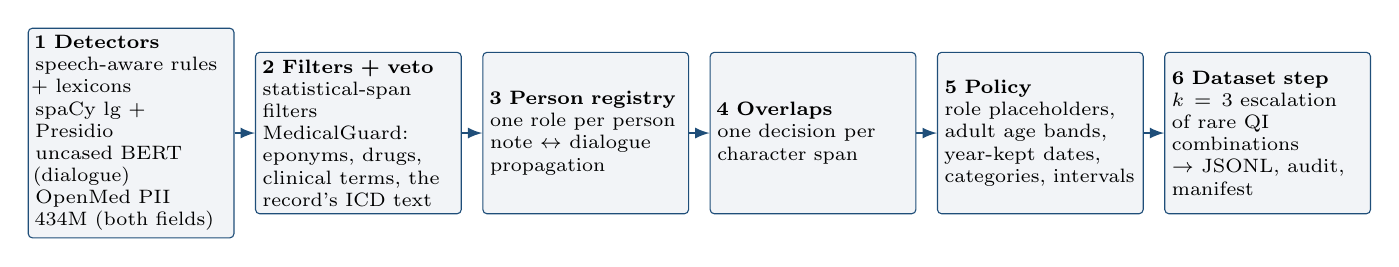
\begin{tikzpicture}[node distance=2.6mm,
  box/.style={draw=accent, fill=accent!6, rounded corners=1.5pt, text width=2.43cm, minimum height=2.05cm,
              align=left, font=\scriptsize, execute at begin node=\nohyph, inner sep=2.6pt},
  arr/.style={-latex, thick, accent}]
\node[box] (a) {\textbf{1 Detectors}\\speech-aware rules + lexicons\\spaCy lg + Presidio\\uncased BERT (dialogue)\\OpenMed PII 434M (both fields)};
\node[box, right=of a] (b) {\textbf{2 Filters + veto}\\statistical-span filters\\MedicalGuard: eponyms, drugs, clinical terms, the record's ICD text};
\node[box, right=of b] (c) {\textbf{3 Person registry}\\one role per person\\note $\leftrightarrow$ dialogue propagation};
\node[box, right=of c] (d) {\textbf{4 Overlaps}\\one decision per character span};
\node[box, right=of d] (e) {\textbf{5 Policy}\\role placeholders, adult age bands, year-kept dates, categories, intervals};
\node[box, right=of e] (f) {\textbf{6 Dataset step}\\$k=3$ escalation of rare QI combinations\\\ra{} JSONL, audit, manifest};
\foreach \x/\y in {a/b,b/c,c/d,d/e,e/f} \draw[arr] (\x) -- (\y);
\end{tikzpicture}
\end{center}

\section{Results}
\textbf{Three kinds of evidence} (1)~\emph{Bosch feedback on an earlier build} (mid-term, before the
hardening and the age-band default): privacy removal proportion 0.5918, ICD-10 F1 delta 0.0, medical concept recall
1.0. It is not a score of this release. (2)~\emph{Local evaluation}: fictional
Synthea worlds with fixed denominators, and aggregate proxies on the 67-record eval split. (3)~\emph{Engineering
acceptance tests} (\S4). 

\textbf{Table 1. What the final hardening changed, on fictional data.} The same synthetic encounters were anonymized
by the code before and after the hardening, both with the age-band policy. dev1 and dev2 are two
Synthea-generated worlds of 300 encounters each; long1 holds 60 records of task-like length. Each cell reads
\emph{before \ra{} after} as count/total: blood pressure was kept exactly in 44 of 92 readings before, and in all 92 after.

{\footnotesize
\begin{tabularx}{\textwidth}{@{}Lccc@{}}
\toprule
Measure & dev1 (300 enc.) & dev2 (300 enc.) & long1 (60 long records)\\
\midrule
\multicolumn{4}{@{}l}{\emph{Clinical content kept: higher is better}}\\
Blood pressure kept exactly & 44/92 \ra{} \textbf{92/92} & 48/91 \ra{} \textbf{91/91} & 18/47 \ra{} \textbf{47/47}\\
Section headers kept & 2793/2806 \ra{} \textbf{2806/2806} & 2717/2737 \ra{} \textbf{2737/2737} & 1145/1163 \ra{} \textbf{1163/1163}\\
Diagnoses, medications and doses, durations & 100\,\% kept, unchanged & 100\,\%, unchanged & 100\,\%, unchanged\\
\midrule
\multicolumn{4}{@{}l}{\emph{Identifying details left in the output: lower is better}}\\
Adults with a bare exact age answer & 31 \ra{} \textbf{0}$^a$ & 29 \ra{} \textbf{0} & 28 \ra{} \textbf{0}$^a$\\
Patients with $\geq3$ children: exact count visible & 20/61 \ra{} \textbf{0/61} & 31/54 \ra{} \textbf{0/54} & 12/16 \ra{} \textbf{0/16}\\
Residual town (of encounters naming one) & 5/104 \ra{} 3/104 & 8/103 \ra{} 4/103 & 2/42 \ra{} 1/42\\
Residual first / last name (unchanged) & 4/162 \textperiodcentered{} 3/261 & 2/156 \textperiodcentered{} 3/251 & 2/52 \textperiodcentered{} 0/60\\
\bottomrule
\end{tabularx}}

$^a$\,Excluding two \code{90+} answers, which are correctly top-coded. In the same comparison, the 12
fictional red-team probes went from 7/12 to \textbf{12/12} privacy and from 39/42 to \textbf{42/42} clinical
assertions; the linkage attack is in Table 2.

\textbf{Table 2. Why adult age bands are the default.} Our synthetic re-identification benchmark (Synthea population,
auxiliary registries, Splink attacker) measured success at a pool of 2,000 under the informed
threat C, where the attacker already knows part of the diagnoses and event years:

{\footnotesize
\begin{tabularx}{\textwidth}{@{}Lcc@{}}
\toprule
Published text & Dev worlds (600 enc., not blind) & Blind world (300 enc., unseen population and phrasing)\\
\midrule
Original & 95.8\,\% & 96.3\,\%\\
MedAnon, exact ages 0--89 & 38.2\,\% & 34.3\,\%\\
MedAnon, adult age bands & 21.5\,\% & 20.3\,\%\\
MedAnon, age bands, hardened code & \textbf{11.7\,\%} & not measured\\
\bottomrule
\end{tabularx}}

With public information only (threat A), success was 0.5\,\% (dev) and 0.0\,\% (blind) even with exact ages. An
independent LLM adversary (local \code{qwen3.5:35b}, the 67 eval records)
points the same way: the expected probability of singling out a patient fell from 0.063 on the original text to
0.034 with exact ages and 0.0042 with age bands. The two attackers model different threats, so we never combine
their numbers.

\textbf{The clinical information loss.} Lab values become clinical intervals by design, and \code{EF [40-50]} straddles the
HFrEF/HFmrEF cut-off. About 9--14\,\% of weights and heights a clinician needs exactly are still generalized on the
Synthea worlds, because the exemptions are rules (paediatrics, weight-based dosing), not clinical understanding. In
an earlier synthetic round, the body-measure step raised the generalized ``must stay exact'' heights from 10/40 to
20/40 and weights from 10/68 to 40/68 (the gold flag is partly inconsistent, but the risk is real). On the older
build, a full human review of the masks (one annotator) found clinical content masked in 25 of the 67 eval
encounters (52 of 518 masked spans). The hardening targets that mechanism; the deterministic audit now flags 3
records instead of 6.

\section{Engineering and reproducibility}
\begin{tight}
\item \textbf{Tests.} 194 automated tests on synthetic data (unit, end-to-end, clinical boundaries, red-team
  regression); 194/194 pass on the GPU host with the production detectors. 
\item \textbf{Offline by construction.} With \code{-{}-offline} nothing touches the network. If a configured model is
  missing, the run stops; it never falls back silently to a weaker pipeline.
\item \textbf{Footprint.} Peak 2,639\,MiB of VRAM including the CUDA context (measured on a 48\,GB card; a physical
  4\,GB card was not tested), 3.64\,GB of RAM; 0.26\,s per record on GPU (0.79\,s for long records), about 13.7\,s
  on CPU.
\item \textbf{Traceability.} Every run writes one audit line per decision, without original text, and a manifest
  with code, config and weight hashes, library versions and input/output hashes. Final eval output: 67/67 valid,
  989 explained decisions, SHA-256 \ldots; the dataset check reports 5/67 records below $k=3$.
\end{tight}

\section{Bonus tasks}
{\footnotesize
\begin{tabularx}{\textwidth}{@{}P{2.6cm}LL@{}}
\toprule
Bonus task & What we built & Evidence\\
\midrule
Adversarial privacy attacks & two independent attackers: a Splink linkage benchmark with three threat models on synthetic worlds, one of them blind (Table 2), and a local LLM adversary (\code{qwen3.5:35b}) that extracts quasi-identifiers and tries to recover masked values & LLM adversary, 67 eval records, age bands: 7 of 98 masked identifiers recovered (7.1\,\%, 95\,\% CI 3.5--14.0); names 2/69, at chance level\\
Explainability & one explanation per decision, including kept medical look-alikes with a reason code; no original text in the audit & 989/989 decisions explained on the final eval output\\
Efficiency & several profiles, from rules + spaCy without torch to the full stack; CPU or GPU & full stack: 0.26\,s per record on GPU, 2,639\,MiB VRAM, 3.64\,GB RAM\\
Without ICD-10 codes & \code{-{}-no-icd} removes the ICD context from the clinical veto & \code{standard} profile: 66/67 eval outputs identical with and without ICD context\\
Robustness to other inputs & synthetic Synthea worlds in other styles: 60 long-form records and a blind world with an unseen population and phrasing & Tables 1 and 2\\
\bottomrule
\end{tabularx}}

\textbf{How the LLM attacker works.} An independent adversary plays an analyst who holds one anonymized
record, US population statistics and a local LLM (\code{qwen3.5:35b}), but no identity database. One schema-constrained call
extracts the patient's quasi-identifiers, each with a verbatim quote; code drops facts whose quote is not in the text,
medical content and restated ICD codes. The remaining facts are priced against population statistics to estimate the
chance of singling the patient out, and a second call guesses what each placeholder hid. On an earlier build with age
bands, no eval record stayed unique in the US population (0/67, against 4/67 originally).

\section{Challenges and ideas that did not work}
{\footnotesize
\begin{tabularx}{\textwidth}{@{}P{3.7cm}LP{4.1cm}@{}}
\toprule
What we tried & What happened & What we did\\
\midrule
GLiNER / GLiNER2 PII models & high synthetic recall, but on real text they relabelled \code{[doctor]} tags and common words as entities & uncased BERT cascade: same recall, 2--4$\times$ cheaper\\
A local LLM as detector (Qwen3.5-2B, Q4) & recall 0.781 against 0.769, at about 57\,s per record on CPU & dropped; no generative model at inference\\
Healthcare-Brain-NER & recall 0.794, no clear gain & not used\\
Threshold-safe lab perturbation ($\pm$3\,\%) & stopped exact joins only: 70.6\,\% of tolerant lab links still succeeded & clinical intervals (11.8\,\%)\\
Exact ages 0--89, Safe-Harbor style & the largest linkage lever in our benchmark (38.2\,\% against 21.5\,\%) & adult decade bands\\
spaCy on vitals lines & ``BP 114/71'' tagged as an organisation: half the synthetic BP readings lost & statistical-span filters (Table 1)\\
\bottomrule
\end{tabularx}}

\section{Limitations and residual problems}
\begin{tight}
\item \textbf{Ambiguous surnames.} Surnames that are also common words (``waters'', ``marks'') can survive a partial
  match: about 1--2\,\% of name mentions on synthetic data. The hardening did not change residual names (Table 1).
\item \textbf{Places without a cue.} Towns mentioned without a residence cue can survive.
\item \textbf{The clinical story is kept on purpose.} ICD-10 codes, event years and the visit year are linkage
  vectors. An attacker who already knows part of the history still re-identifies about 12\,\% of synthetic dev
  encounters.
\item \textbf{Children.} Exact paediatric ages and children's birth years are kept because they matter clinically.
\item \textbf{Not formal $k$-anonymity.} The $k=3$ step covers four quasi-identifier types only; 5/67 eval records
  stay below $k=3$.
\end{tight}

\section{Conclusion}
In the encounters most of the identifying power sits in age, family, work,
places and the clinical story, and the medical vocabulary is full of person-like words. We combined off-the-shelf models
with parts built for this data: the note-guided truecasing of the dialogue, the name-dominance ratio, the ICD-aware
clinical veto, the cross-field person registry, per-decision explanations, and a re-identification benchmark with
three threat models that chose the policy. This let us make each trade-off deliberately, measure it on fixed
denominators and explain every decision. It cannot make a rich clinical history anonymous on its own; we measured that residual risk
and report it rather than hide it.

\textbf{AI tools disclosure.} We used Claude (Anthropic, through Claude Code) and other AI coding assistants
extensively for implementation, tests, analysis and documentation, including drafts of this report. Their output was
checked by the automated tests, controlled synthetic benchmarks and human review, and every number above traces to a
script, test or manifest in the repository. The anonymizer uses no generative model; a local LLM appears only in the
adversarial attack code (\code{attack/}).

{\raggedright\textbf{Team.} \mbox{Matteo Marello (\href{mailto:matteomarello3@gmail.com}{matteomarello3@gmail.com})} \textperiodcentered{}
\mbox{Paolo Pusterla (\href{mailto:pusterlapaolo81@gmail.com}{pusterlapaolo81@gmail.com})} \textperiodcentered{}
\mbox{Tommaso Riggio (\href{mailto:tommy.riggio204@gmail.com}{tommy.riggio204@gmail.com})} \textperiodcentered{}
\mbox{Andrea Orione (\href{mailto:andrea.orione02@gmail.com}{andrea.orione02@gmail.com})} \textperiodcentered{}
\mbox{Valeria Intini (\href{mailto:valeriaintini2001@gmail.com}{valeriaintini2001@gmail.com})}.
Code released under the MIT licence. Evidence: \code{reports/FINAL\_HARDENING.md}, \code{research/reid/}, \code{attack/paper/}.\par}

\end{document}
